%%%%%%%%%%%%%%%%%%%%%%%%%%%%%%%%%%%%%%%%%%%%%%%%%%%%%%%%%%%%%%%%%%%%%%%%%%%%%%%%
% Uncertainties and Results:
%%%%%%%%%%%%%%%%%%%%%%%%%%%%%%%%%%%%%%%%%%%%%%%%%%%%%%%%%%%%%%%%%%%%%%%%%%%%%%%%
\chapter{Statistical Analysis, Uncertainties, and Results}
\label{statAnalysis_uncerts_results}
%%%%%%%%%%%%%%%%%%%%%%%%%%%%%%%%%%%%%%%%%%%%%%%%%%%%%%%%%%%%%%%%%%%%%%%%%%%%%%%%
After estimating the background, the $\Mlljj$ distributions found in the selected data and predicted background events 
were compared.  The difference between the number of data and background events was compared to the background uncertainty, 
the predicted number of simulated \WR events, and the \WR prediction uncertainty (simulation details in Appendix \ref{app_wrMC}).  
The $\Mlljj$ distribution found in simulated \WR events was several hundred $\GeV$ wide or larger (Figure 
\ref{fig:signalShapes}), so excesses of data events above the background can be consistent with several \mWR hypotheses.  
A set of $\Mlljj$ windows, each tailored to the $\Mlljj$ distribution of a specific \mWR hypothesis, was used to interpret 
the excesses of data in the context of different \mWR hypotheses.  The sizes of these windows, the uncertainties on 
the number of signal and background events, and the results of the comparisons were determined using the procedures described 
here.

\begin{figure}
	\centering
	\begin{subfigure}[t]{2.4in}
		\centering
		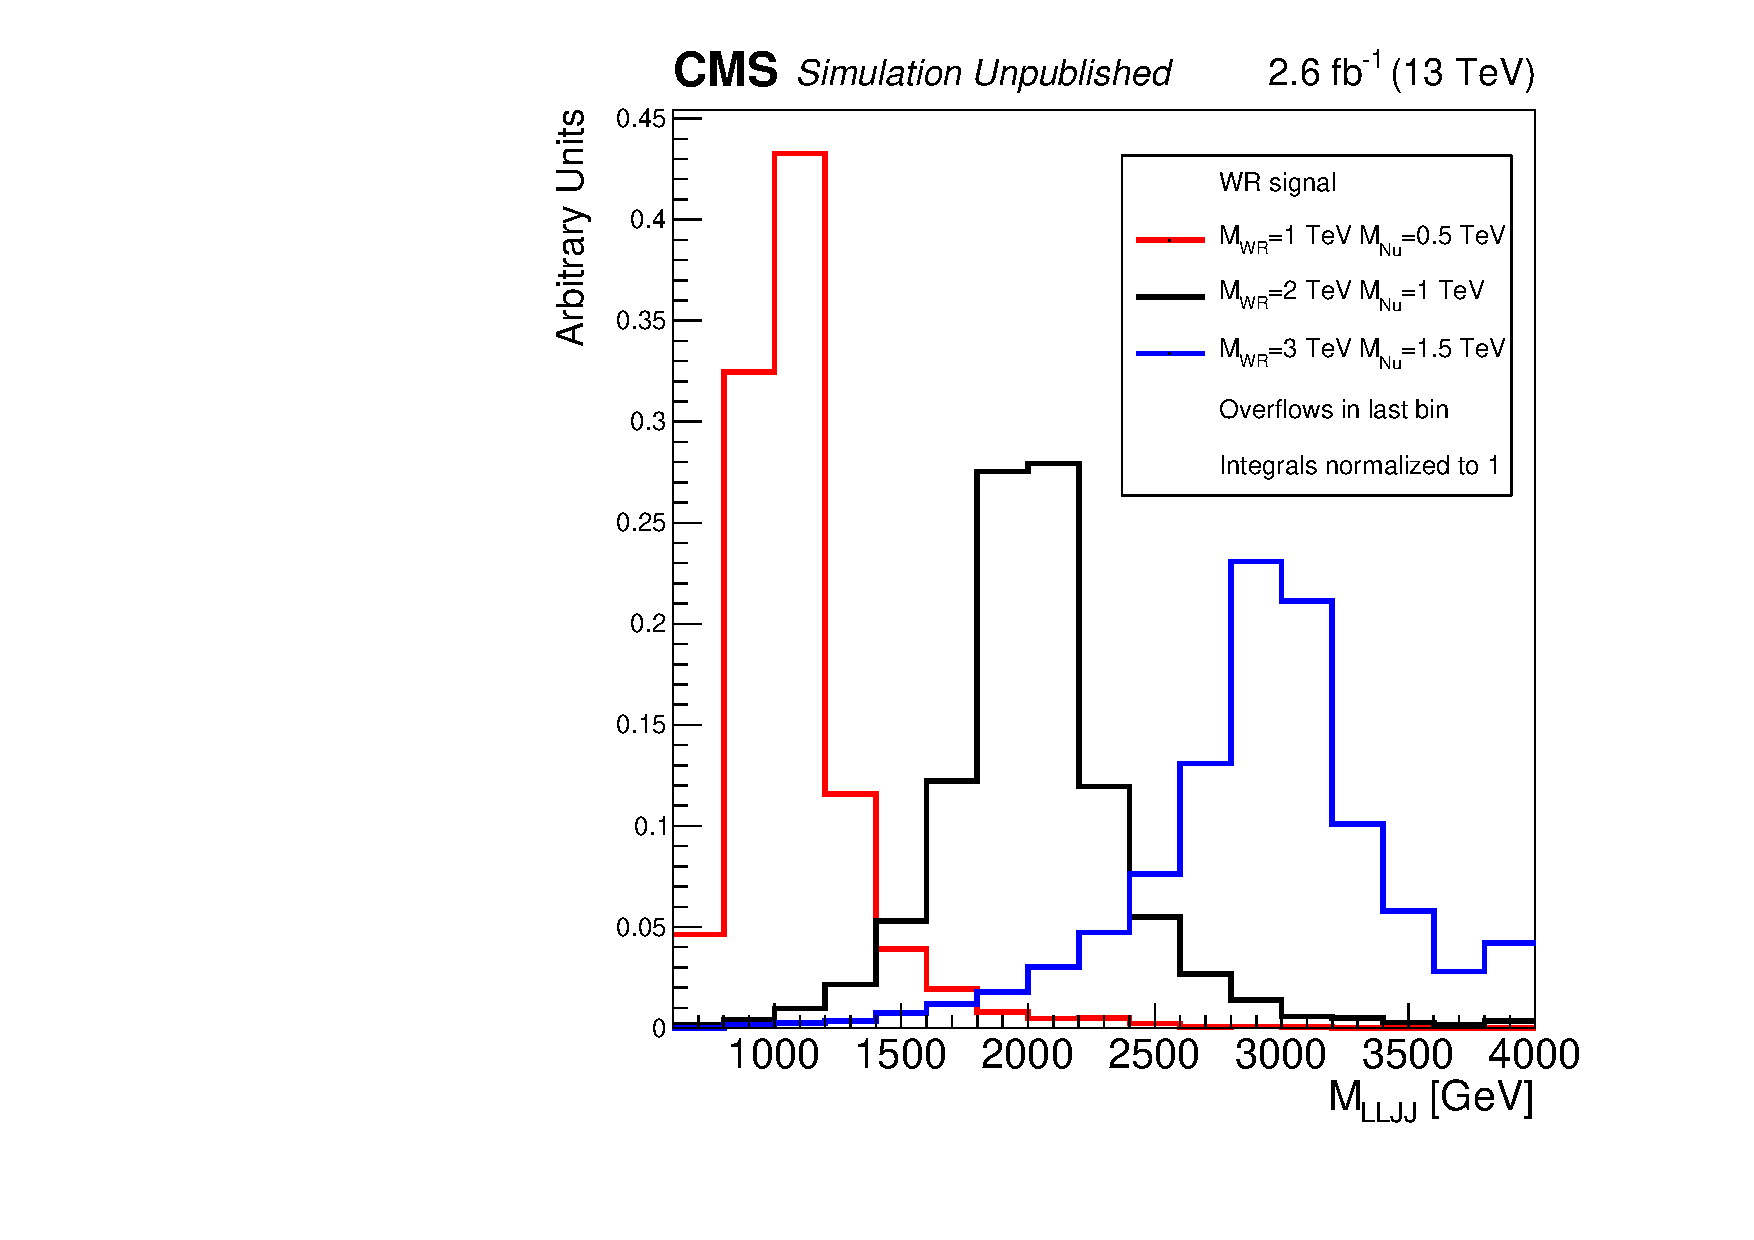
\includegraphics[width=2.4in]{figures/Mlljj_signalRegionCuts_severalWrSignals_EE.pdf}
	\end{subfigure}
	\thickspace
	\begin{subfigure}[t]{2.4in}
		\centering
		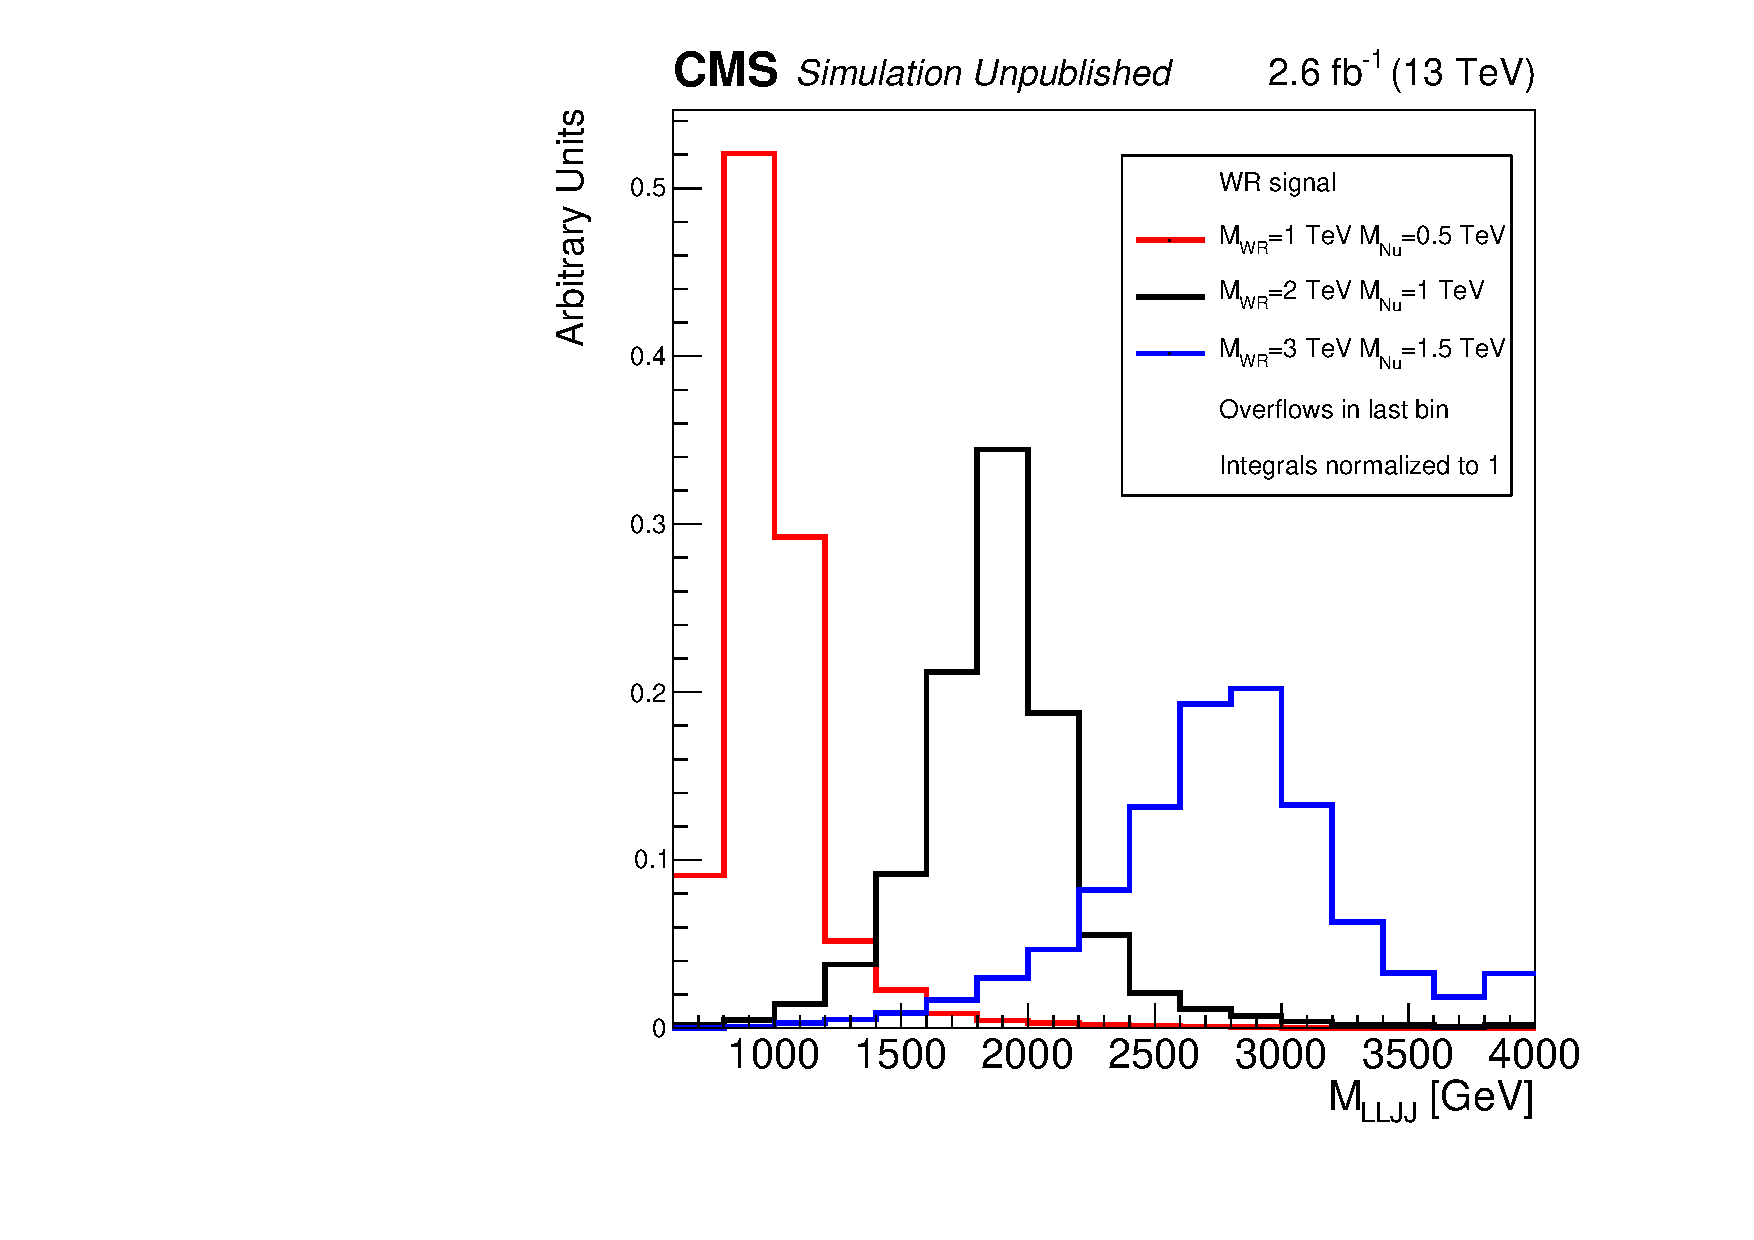
\includegraphics[width=2.4in]{figures/Mlljj_signalRegionCuts_severalWrSignals_MuMu.pdf}
	\end{subfigure}
	\caption{The $\Mlljj$ distribution found in selected \WR events with different \mWR and \mnul.  The $ee$-channel is on the 
	left, and the $\mu\mu$-channel is on the right.}
	\label{fig:signalShapes}
\end{figure}


%%%%%%%%%%%%%%%%%%%%%%%%%%%%%%%%%%%%%%%%%%%%%%%%%%%%%%%%%%%%%%%%%%%%%%%%%%%%%%%%
% Statistical Analysis 
%%%%%%%%%%%%%%%%%%%%%%%%%%%%%%%%%%%%%%%%%%%%%%%%%%%%%%%%%%%%%%%%%%%%%%%%%%%%%%%%
\section{Statistical Analysis}
\label{sec:statAnalysis}
%%%%%%%%%%%%%%%%%%%%%%%%%%%%%%%%%%%%%%%%%%%%%%%%%%%%%%%%%%%%%%%%%%%%%%%%%%%%%%%%
The number of $\Mlljj$ windows was chosen based on how the $\Mlljj$ distribution found in selected 
simulated \WR events changed with \mWR and \mnul.  For a fixed \mWR, the shape of the $\Mlljj$ distribution found in signal 
events is weakly dependent on \mnul (Figure \ref{fig:mWrShapeVsMNu}), only because the $\WR \rightarrow \ell\ell jj$ cross 
section $\times$ branching ratio varies weakly with \mnul.  Since the shape varies weakly with \mnul, one $\Mlljj$ window is 
assigned per \mWR, independent of \mnul.  The $\Mlljj$ window size for a specific \mWR is determined using events that have 
$\mnul = \frac{1}{2}\mWR$, because at this $\mnul$ the event selection efficiency is maximized or nearly maximized.  As \mWR 
increases the $\Mlljj$ distribution shape shifts to higher values, and the distribution normalization 
decreases with the \WR cross section $\times$ branching ratio.  However, for $X \geq 2.0$ $\TeV$, the $\Mlljj$ distributions 
found in signal events that have $\mWR = X$ and $\mWR = X + 0.2$ $\TeV$ overlap by 10\% or more (Figure \ref{fig:mWrShapeVsMWr}).  
The two $\Mlljj$ windows that are used for $\mWR = X$ and $\mWR = X + 0.2$ $\TeV$ are sensitive to signals that have 
$X < \mWR < X + 0.2$ $\TeV$, so finer granularity in \mWR is not needed.  To cover the entire $\Mlljj$ spectrum found in the 
data, one $\Mlljj$ window is assigned to each value of \mWR stepping from 0.8 to 6 $\TeV$ in increments of 0.2 $\TeV$.  The size 
of each $\Mlljj$ window was determined based on the shape and normalization of the $\Mlljj$ distribution found in background 
events.  Specifically, each window's size was chosen to maximize the difference between the number of signal and background 
events, and thus minimize the upper limit on the \WR cross section $\times$ branching ratio.

\clearpage
\begin{figure}[h]
	\centering
	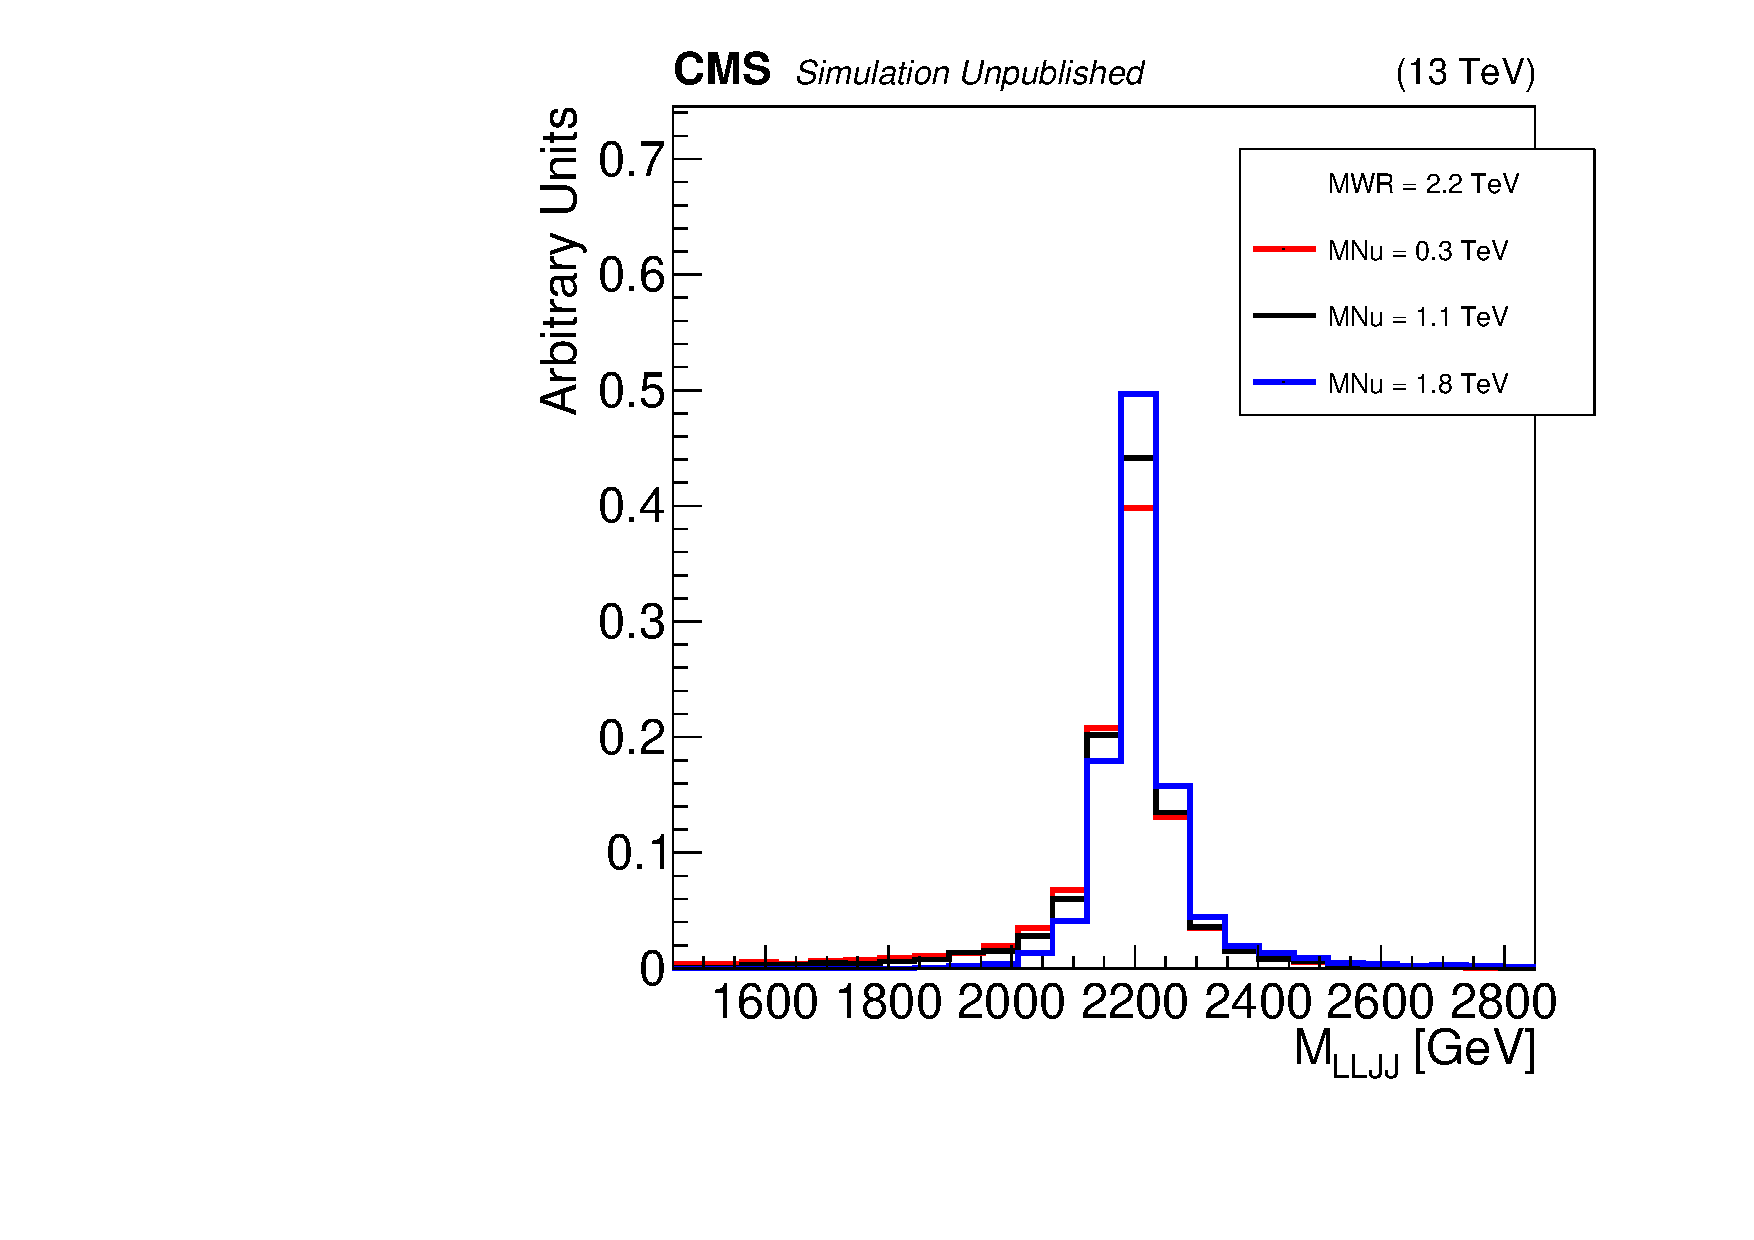
\includegraphics[width=0.45\textwidth]{figures/massGenFstHvyPtcl_MWR_2200_several_MNu_private.pdf}
	\caption{The $\Mlljj$ distribution found in $\WR \rightarrow \ell\ell jj$ events that have $\mWR = 2.2$ $\TeV$ 
	and different \mnul.}
	\label{fig:mWrShapeVsMNu}
\end{figure}

\begin{figure}[h]
	\centering
	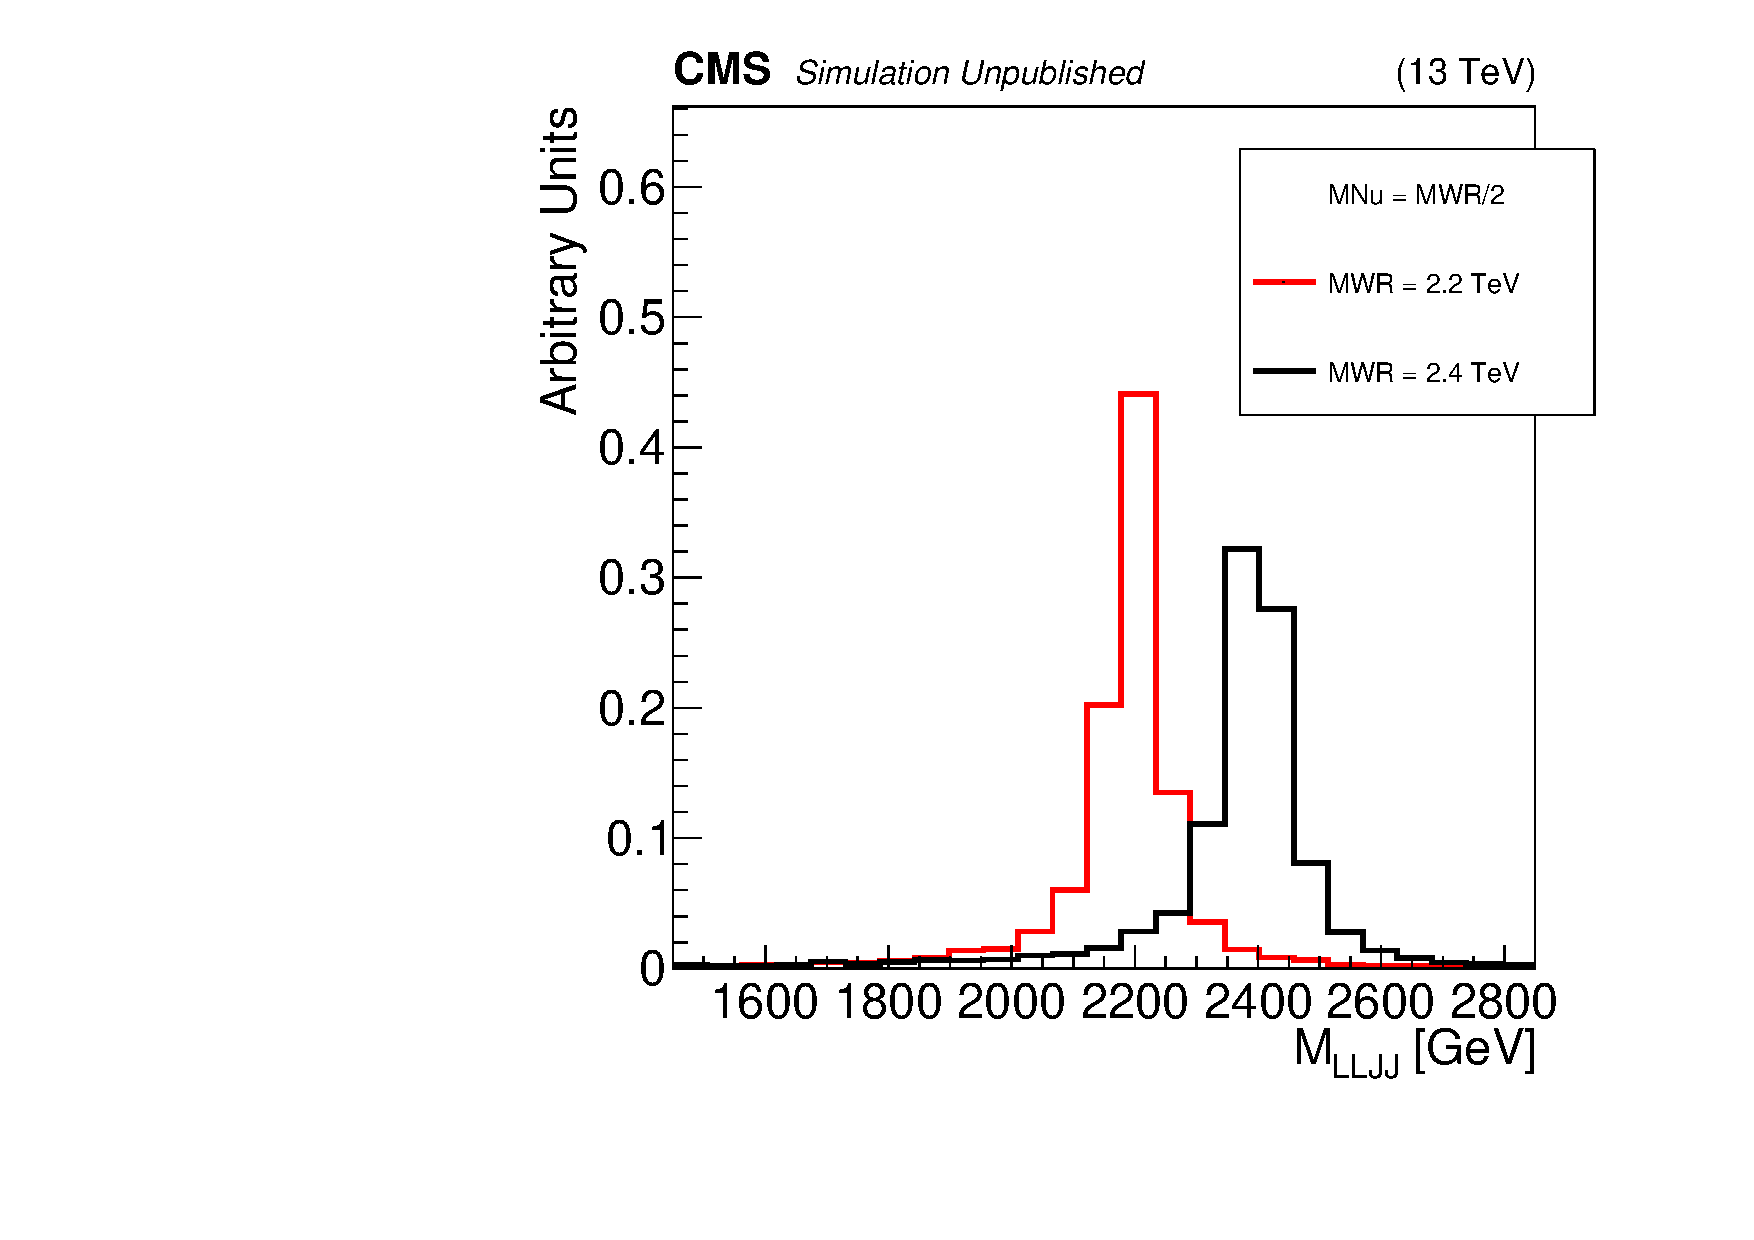
\includegraphics[width=0.45\textwidth]{figures/massGenFstHvyPtcl_several_MWR_and_MNu_private.pdf}
	\caption{The $\Mlljj$ distribution found in $\WR \rightarrow \ell\ell jj$ events that have $\mnul = \frac{1}{2}\mWR$ 
		and different \mWR.}
	\label{fig:mWrShapeVsMWr}
\end{figure}
\clearpage

\subsection{Bayesian Limits}
\label{sec:bayesianStatsAndLimits}
The \WR cross section $\times$ branching ratio ($\sigma(\WR) \times BR(\WR \rightarrow \ell\ell jj)$) limits are calculated 
using several quantities.  Each limit for a specific \mWR signal is calculated using the number of measured events $G$ and 
predicted signal ($S$) and background ($B$) events in the $\Mlljj$ window, and their uncertainties $\delta S$ and $\delta B$.  
Expected limits, calculated by setting $G = B$, were used to determine the sizes of the $\Mlljj$ bins.  Expected limits were 
calculated at 95\% confidence level (CL) using a Poisson model of the $S \plus B$ events:

\begin{equation}
	Poisson(\mu S(\pmb{\theta}) \thickspace \plus \thickspace B(\pmb{\theta}))
	\label{eq:poissonModel}
\end{equation}
where $\mu$ is the dimensionless \WR signal strength, and $\pmb{\theta}$ represent the uncertainties $\delta S$ and $\delta B$ 
described later in Section \ref{sec:uncertainties}.  Using Bayesian statistics, the probability distribution for $\mu$ given 
$G$ measured events, $p(\mu|G)$, is obtained by evaluating the integral \cite{bayesianDataAnalysis}:

\begin{equation}
	p(\mu|G) = \int p(\mu|\pmb{\theta},G)p(\pmb{\theta}|G)d\pmb{\theta}
	\label{eq:sigStrngthProbDist}
\end{equation}
where $p(\pmb{\theta}|G)$ are the probability distributions for the uncertainties given the measurement $G$ (``marginal 
posterior distributions''), and $p(\mu|\pmb{\theta},G)$ are the probability distributions for $\mu$ given the uncertainties, 
and the measurement $G$ (``conditional posterior distributions'').  Functional forms of the marginal posterior distributions 
are either log-normal or Gamma distributions depending on the uncertainty, and are identified later for specific uncertainties.  
Functional forms of the conditional posterior distributions are derived from uniform prior distributions and Equation 
\ref{eq:poissonModel}.  The integrals in Equation \ref{eq:sigStrngthProbDist} were evaluated numerically using \MC methods 
to derive $p(\mu|G)$.  Then, $p(\mu|G)$ was integrated from $\mu =$ 0 to $\mu = \mu_{max}$ such that the normalized integral 
equaled 0.95.  The value $\mu_{max}$ is the 95\% CL upper limit on the signal strength.  The value of $\sigma(\WR) \times 
BR(\WR \rightarrow \ell\ell jj)$ obtained from simulations is multiplied by $\mu_{max}$ to calculate the upper limit on 
$\sigma(\WR) \times BR(\WR \rightarrow \ell\ell jj)$.

\subsection{$\Mlljj$ Window Sizes}
\label{sec:mlljjWindows}
The sizes of the $\Mlljj$ windows were chosen to minimize the 95\% CL upper limit on $\sigma(\WR) \times BR(\WR \rightarrow \ell\ell jj)$.  
For each value of \mWR between 0.8 and 6 $\TeV$, the size of the corresponding window was determined using the following 
procedure:

\begin{itemize}
	\item 150 $\Mlljj$ windows of different sizes and central values were defined based on the peak position in the \WR $\Mlljj$ 
		distribution.  The window lower bound went down to 40\% of \mWR, and the upper bound went up to 140\% of \mWR.
	\item For each window:
	\begin{itemize}
		\item The number of signal events $S$ and background events $B$ were counted.
		\item A Poisson distribution was created with mean $B$, and a random number $C$ was pulled 
			from the Poisson distribution.  $C$ represents the number of measured events in the window.
		\item Using $C$, $S$, $B$, and the procedure described in Section \ref{sec:bayesianStatsAndLimits}, an 
			expected upper limit on $\sigma(\WR) \times BR(\WR \rightarrow \ell\ell jj)$ was calculated at 
			95\% CL.  The systematic uncertainties on $S$ and $B$ had a negligible effect on the final 
			window size, so only the statistical uncertainties on $S$ and $B$ were included.
		\item The limit was recalculated 300 times, and each time a new random number $C$ was pulled 
			from the Poisson distribution.  The median value of all 300 limits is the expected upper limit 
			for the window.
	\end{itemize}
	\item The window that minimized the expected upper limit was chosen.
\end{itemize}

The $\Mlljj$ windows, listed in Table \ref{tab:masscuts}, capture at least 70\% of the corresponding \WR $\Mlljj$ distribution.  
The central value of each window ($\frac{max \plus min}{2}$) exceeds the corresponding \mWR value to minimize the predicted 
background, which falls rapidly with increasing $\Mlljj$.

\begin{table}[h]
\caption{$\Mlljj$ window ranges that minimized the expected upper limit on the \WR cross section at different \mWR values.}
\label{tab:masscuts}
\centering
\begin{tabular}{|c|r@{ - }l|r@{ - }l|} \hline
\mWR (\GeV) & \multicolumn{4}{c|}{\Mlljj window (\GeV)}  \\\hline
& \multicolumn{2}{c|}{Electrons}  & \multicolumn{2}{c|}{Muons}  \\  \hline
 800  & 700       &  1100       &  700       &  1200      \\  \hline
1000  & 900       &  1300       &  900       &  1400      \\  \hline
1200  & 1100       &  1550       &  1100       &  1650      \\  \hline
1400  & 1250       &  1750       &  1300       &  1850      \\  \hline
1600  & 1450      &  2000       &  1500      &  2100      \\  \hline
1800  & 1600      &  2250       &  1600      &  2300      \\  \hline
2000  & 1850      &  2550       &  1850      &  2600      \\  \hline
2200  & 2000      &  2800       &  2000      &  2850      \\  \hline
2400  & 2150      &  3100       &  2150      &  3100      \\  \hline
2600  & 2250      &  3400       &  2300      &  3400      \\  \hline
2800  & 2350      &  3700       &  2400      &  3700      \\  \hline
3000  & 2500      &  4000       &  2500      &  3950      \\  \hline
3200  & 2550      &  4300       &  2700      &  4250      \\  \hline
3600  & 2700      &  4900       &  2900      &  4850      \\  \hline
3800  & 2750      &  5200       &  2950      &  5150      \\  \hline
4000  & 2800      &  5500       &  3000      &  5450      \\  \hline
4200  & 2800      &  5750       &  3100      &  5750      \\  \hline
4400  & 2850      &  6050       &  3150      &  6100      \\  \hline
4600  & 2850      &  6300       &  3150      &  6400      \\  \hline
4800  & 2850      &  6600       &  3200      &  6700      \\  \hline
5000  & 2900      &  6850       &  3200      &  7000      \\  \hline
5200  & 2900      &  7050       &  3200      &  7300      \\  \hline
5600  & 2900      &  7500       &  3200      &  7850      \\  \hline
5800  & 2950      &  7700       &  3200      &  8150      \\  \hline
6000  & 2950      &  7900       &  3200      &  8400      \\  \hline
\end{tabular}
\end{table}


%%%%%%%%%%%%%%%%%%%%%%%%%%%%%%%%%%%%%%%%%%%%%%%%%%%%%%%%%%%%%%%%%%%%%%%%%%%%%%%%
% Uncertainties 
%%%%%%%%%%%%%%%%%%%%%%%%%%%%%%%%%%%%%%%%%%%%%%%%%%%%%%%%%%%%%%%%%%%%%%%%%%%%%%%%
\section{Uncertainties}
\label{sec:uncertainties}
%%%%%%%%%%%%%%%%%%%%%%%%%%%%%%%%%%%%%%%%%%%%%%%%%%%%%%%%%%%%%%%%%%%%%%%%%%%%%%%%
In each window, the observed limit, using data, and the expected limit were calculated with all systematic and statistical 
uncertainties included.  The dominant uncertainties were the 40\% $\DY$+jets uncertainty, the lepton and jet energy 
uncertainties, and the top quark background statistical uncertainty.  The magnitudes of these uncertainties and all 
others that affected the number of predicted signal and background events were calculated in each $\Mlljj$ window using the 
procedures described here.  The uncertainty magnitude is the same for all $\Mlljj$ windows unless noted otherwise.

\subsection{Energy and Lepton Identification Uncertainties}
\label{sec:enrgyLeptIdUncs}
The lepton and jet energy uncertainties are unique in that they are the only uncertainties that can change the shapes of 
the $\Mlljj$ distributions found in signal and background events.  These uncertainties, specifically on the lepton and 
jet energy scales and resolutions, affect the energies of all reconstructed leptons and jets in every event.  Variations 
of lepton and jet energies within their uncertainties can cause each event to pass or fail the selection criteria, or 
change a selected event's $\Mlljj$ value.  The jet energy uncertainties went up to 25\% for jets that had low $\pt$ and 
large $|\eta|$, and the lepton energy uncertainties went up to $\sim$7\% for electrons and muons.  The efficiency of the 
lepton ID selection criteria is sensitive to lepton and jet energies, so the energy uncertainties are correlated with the 
lepton ID selection efficiency uncertainty.  The effect of energy and lepton ID uncertainties were estimated simultaneously 
using the following procedure:

\begin{itemize}
	\item In each event selected by a trigger, but before applying any lepton or jet selection criteria:
	\begin{itemize}
		\item Eight random numbers were pulled from eight different Gaussians, each with mean 0 and variance 1.
		\item Two random numbers multiplied each electron's energy scale and resolution uncertainty to determine the 
			energy change applied to each electron.  In simulated events, a third random number multiplied 
			each electron's ID weight uncertainty, and the change in weight of the two selected electrons was propagated 
			to the total event weight.
		\begin{itemize}
			\item Using the same procedure with three other random numbers, the effect of muon energy and ID uncertainties 
				were propagated to each muon's energy and ID weight.
		\end{itemize}
		\item The last two random numbers multiplied every jet's energy scale and resolution uncertainty, and these 
			energy changes were added to the jet's energy.
	\end{itemize}
	\item The offline selection criteria were applied to each event.  Selected events were assigned to $\Mlljj$ 
		bins based on their $\Mlljj$ values.
\end{itemize}

This procedure was repeated 3200 times for every event used to predict the signal and background $\Mlljj$ distributions.  
Then, a distribution was made showing the number of selected events in each window for all 3200 iterations (Figure 
\ref{fig:effectOfEnergyIdUncerts}).  The distribution's standard deviation is the uncertainty on the number of predicted 
events, and this uncertainty depended on the $\Mlljj$ window.  Increasing the \mWR hypothesis from 1.8 to 4.0 $\TeV$, the 
uncertainty in each $\Mlljj$ window on the signal prediction was constant - 1\% in the $ee$-channel, and 3\% in the 
$\mu\mu$-channel.  In both channels over the same \mWR range the uncertainty on the \DY prediction increased from 10\% to 
20\%, and the uncertainty on the top quark prediction increased from 14\% to 53\%.  These uncertainties were included in 
limit calculations using Gamma distributions for the marginal posterior distributions.

\begin{figure}[h]
	\centering
	
\includegraphics[width=1.0\textwidth]{figures/missingImage.png}
	\caption{The number of expected $\WR \rightarrow \mu\mu jj$ signal events with $\mWR = 2.2$ $\TeV$ in the 2.2 $\TeV$ 
	$\Mlljj$ window after 3200 iterations of energy and ID uncertainty variations.}
	\label{fig:effectOfEnergyIdUncerts}
\end{figure}

%\begin{table}[ht]
%	\caption{The effect of energy and ID uncertainties on the number of signal and background events in the $\Mlljj$ 
%		window optimized for the $\mWR = 2.2\TeV$ hypothesis.  All uncertainties are in percentages of expected events.  The top 
%	quark background estimate is sensitive to both the $e$ and $\mu$ energy uncertainties.}
%  \label{tab:impactOfEnergyIdUncerts}
%  \centering
%    \begin{tabular}{c|c|c|c}
%		Process & Uncertainty sources    & $\Delta(\Neejj)$ (\%) & $\Delta(\Nmumujj)$ (\%)  \\
%      \hline
%	  \WR & lepton energy and ID & $1$ & $3$ \\ 
%	  \WR & jet energy & $1$ & $1$ \\ 
%	  \DY &  lepton energy and ID & $4$ & $7$  \\
%	  \DY &  jet energy & $14$ & $11$  \\
%	 Top quark background & lepton energy & $8$ & $8$ \\
%	 Top quark background & jet energy & $2$ & $2$  \\
%  \hline
%  \end{tabular}
%\end{table}


\subsection{Statistical Uncertainty}
\label{sec:statUnc}
The signal and background statistical uncertainties were calculated as $\sqrt{\sum w_{i}^{2}}$, where $w_{i}$ is the weight 
of event i, and the sum ran over all events in a $\Mlljj$ window.  The $e\mu$ data events, used to estimate the top quark 
background, all have a weight of 1.  The simulated \WR and $\DY$+jets event weights were normalized to the integrated 
luminosity of the data, and as a result have positive weights less than 1.  The statistical uncertainty due to the number 
of selected events was higher for the background prediction than the signal prediction, and the background uncertainty 
depended on the $\Mlljj$ window.  Increasing the \mWR hypothesis from 1.8 to 4.0 $\TeV$, the uncertainty in each $\Mlljj$ 
window on the signal prediction was 1\% in both channels.  In both channels over the same \mWR range the uncertainty on the \DY 
prediction increased from 10\% to 13\%, and the uncertainty on the top quark prediction increased from 38\% to 100\%.  The 
statistical uncertainty was the largest uncertainty on the top quark background prediction.  These uncertainties were included 
in limit calculations using Gamma distributions for the marginal posterior distributions.

No $e\mu$ data events were found in data with $\Memujj \geq 2700$ $\GeV$, so in $\Mlljj$ windows used for $\mWR \geq 3.6$ $\TeV$ 
the top quark background prediction was 0 events.  In these mass windows the statistical uncertainty on the top quark prediction 
was set to 1 $e\mu$ event multiplied by the appropriate $\ell\ell:e\mu$ normalization factor - 0.659 or 0.432.

%\begin{table}[ht]
%	\caption{Impact of statistical uncertainty on the number of expected signal and background events in the $\Mlljj$ 
%		window optimized for the $\mWR = 2.2\TeV$ hypothesis.  All uncertainties are in percentages of expected events.}
%  \label{tab:impactOfStatUncert}
%  \centering
%    \begin{tabular}{c|c|c}
%		Process & $\Delta(\Neejj)$ (\%) & $\Delta(\Nmumujj)$ (\%)  \\
%      \hline
%	  \WR & $1$ & $1$ \\
%	  \DY & $6$ & $5$ \\
%	 Top quark background & $44$ & $44$  \\
%  \hline
%  \end{tabular}
%\end{table}

\subsection{Background Uncertainty from Control Regions}
\label{sec:bkgndNormUnc}
As discussed previously (Chapter \ref{sec:backgroundEstimation}), the shape of the $\Mlljj$ distribution found in simulated 
background events in control regions motivated assigning additional uncertainties.  Based on the variation of 
$\frac{\ell\ell}{e\mu}$ top quark events versus $\Mlljj$, a 10\% uncertainty was assigned to the top quark background prediction.  
Based on the disagreement in the $\Mlljj$ distribution between data and and simulated $\DY$+jets events selected in the low 
$\Mll$ control region, a 40\% uncertainty was assigned to the \DY background prediction.  This was the dominant uncertainty 
on the \DY background prediction.  Both uncertainties were included in limit calculations using log-normal distributions for 
the marginal posterior distributions.

\subsection{Lepton Reconstruction and Trigger Efficiency Uncertainties}
\label{sec:leptonRecoTriggerEffUnc}
The efficiencies of lepton reconstruction algorithms and muon trigger selection criteria differed between data and simulated 
events, and these differences were corrected by applying $\sim$unity event weights to simulated events.  The uncertainties on 
these weights affected the signal and \DY background predictions.  In the $\mu\mu$-channel, 
the trigger and lepton reconstruction efficiency weights varied with the $\pt$ and $\eta$ of the selected muons, and their 
uncertainties were statistical - based on the number of data and simulated events used to calculate the weights.  The uncertainty 
on the muon reconstruction weight was negligible.  For events triggered by muons that had $\pt < 140$ $\GeV$, the muon trigger 
weight uncertainty resulted in an uncertainty below 0.5\% on the signal and \DY predictions.  For events triggered by higher $\pt$ 
muons, when the triggering muon had $|\eta| < 2.1$ the prediction uncertainty was below 3\%, and for higher $|\eta|$ muons the 
uncertainty was 5.1\%.  For events that passed the $ee$-channel criteria, an electron reconstruction efficiency weight of 0.982 
was applied to all selected electrons, and propagated into the weight of each event.  The reconstruction weight uncertainty, 
calculated as the maximum difference between 0.982 and an $\Et,\eta$ dependent weight, resulted in a 2\% uncertainty on the 
signal and \DY predictions.  The lepton reconstruction and trigger uncertainties were included in limit calculations using 
log-normal distributions for the marginal posterior distributions.

\subsection{Cross Section, Luminosity, Pileup and PDF Weight Uncertainties}
\label{sec:crossSxnPileupPdfUnc}
Additional weights were applied to simulated \WR and $\DY$+jets events for several reasons.  The uncertainties on these weights 
resulted in additional, albeit small, uncertainties to the signal and \DY background predictions.

Simulated events were weighted by the integrated luminosity of data $\Ell$, the cross section $\sigma$, and the number of 
simulated events $N_{evts}$: $\frac{\Ell \times \sigma}{N_{evts}}$.  The uncertainty on the integrated luminosity measurement 
resulted in a 2.7\% uncertainty on the signal and \DY predictions.  The uncertainty on the \DY cross section resulted in a 
2\% uncertainty on the \DY prediction in the $ee$-channel, and a 1\% uncertainty in the $\mu\mu$-channel.  The uncertainty on 
the \WR cross section, calculated during simulations of \WR events, resulted in an uncertainty below 0.5\% on the signal 
prediction for all values of \mWR.

The efficiency to reconstruct an interaction as a vertex was known exactly in simulated events, but could only be estimated 
to within $\sim$5\% uncertainty in data events.  As a result, there was an uncertainty on the number of pileup interactions 
reconstructed in each data event.  Simulated events were weighted to bring the pileup distributions found in data and simulated 
events into agreement, ignoring the pileup uncertainty in data.  The effect of the pileup uncertainty on the signal and 
background predictions was estimated by shifting the pileup distribution found in data within its uncertainty, and calculating 
new weights for simulated events.  The change in the signal and \DY predictions using the new and original weights was taken 
as an uncertainty.  The resulting uncertainty for signal and \DY predictions was between 2\% and 3\% for all $\Mlljj$ windows.

In simulated events, the distribution of momenta amongst gluons, up, down, and strange quarks, and their anti-quarks in interacting 
protons was modeled using one parton distribution function (pdf).  \DY events were simulated using the NNPDF30 pdf \cite{nnpdf30}, 
and signal events were simulated using the NNPDF23 pdf \cite{nnpdf23}.  Both pdfs are parameterized in terms of the independent 
variables x (momentum fraction) and $Q_{0}^{2}$ (energy scale), and several constant coefficients and exponents whose values 
and uncertainties are determined using experimental data.  In each simulated event these coefficients and exponents were varied 
within their uncertainties, and the average change in the cross section was propagated to the event weight.  The average change 
in the total weight of all events was taken as an uncertainty on the signal or \DY prediction.  The uncertainty on the \DY 
prediction was between 2\% and 3\% for all $\Mlljj$ windows.  As \mWR increased from 0.8 to 4 $\TeV$ the uncertainty on the signal 
prediction increased from 1\% to 15\%.  The portion of the \WR pdf uncertainty that affected the $(\eta,\phi)$ trajectories was 
below 1\% for all values of \mWR; only this portion of the uncertainty was included in limit calculations.  The remaining 
uncertainty, that grew with \mWR, depended on unconstrained parameters of the LRS model, and therefore was not included in limit 
calculations.


In each simulated pp interaction the coupling $\alpha_{QCD}$ was calculated at the renormalization energy scale $\mu_{R}$, and 
QCD interactions were divided into two regions based on a factorization energy scale $\mu_{F}$.  QCD interactions that exchanged 
momentum $Q^{2} \ll \mu_{F}^{2}$ are not perturbative in $\alpha_{QCD}$, and are simulated using low energy QCD models.  QCD 
interactions that exchanged momentum $Q^{2} \gtrsim \mu_{F}^{2}$ are simulated using perturbative QCD \cite{qcdFactorizationTheory}.  
Neither $\mu_{R}$ nor $\mu_{F}$ are extracted from experimental data or simulations, and no uncertainties are assigned to either 
parameter.  Variations of $\mu_{R}$ or $\mu_{F}$ affect the simulated cross section, and therefore the signal and \DY 
predictions.  The signal and \DY prediction uncertainties due to variations in $\mu_{R}$ and $\mu_{F}$ were estimated by 
simulating each event 8 different times, each time increasing or decreasing one or both parameters by a factor of 2.  Then, the 
change in cross section was propagated to the weight of each event.  The maximum change in the total weight of all selected events 
relative to the standard $\mu_{R}$ and $\mu_{F}$ values was taken as an uncertainty on the prediction.  The uncertainties on the 
signal and \DY predictions were below 3\%.

These uncertainties on the signal and \DY predictions were included in limit calculations using log-normal distributions for the 
marginal posterior distributions.

%\begin{table}[ht]
%	\caption{The uncertainty ($\Delta$) in the number of \WR events ($\Nlljj$) due to PDF and QCD scale uncertainties.}
%  \label{tab:wrPdfAndQCDscaleUnc}
%  \centering
%    \begin{tabular}{c|c|c}
%		\mWR ($\GeV$)             & $\Delta(\Neejj)$ (\%) & $\Delta(\Nmumujj)$ (\%)  \\
%      \hline
%	  1000  & $4$ & $4$ \\
%	  2200 & $7$ & $7$ \\
%	  3000 & $15$ & $15$ \\
%	  4000 & $18$ & $19$ \\
%	  \hline
%  \end{tabular}
%\end{table}

\subsection{Cumulative Uncertainty}
\label{sec:cumulativeUnc}
The cumulative effect of all uncertainties on the number of ST background and \WR signal events in several $\Mlljj$ windows is 
shown in Table \ref{tab:expectedEventsAndAllUncs}.  All uncertainties excluding the statistical uncertainty are labeled as systematic 
uncertainties, and the magnitudes of all systematic uncertainties are summed in quadrature.  The dominant \DY background uncertainty 
was the 40\% uncertainty assigned based on disagreement between data and simulated ST backgrounds in a control region where good 
agreement was expected.  The dominant top quark background uncertainty was the statistical uncertainty, as fewer than 500 $e\mu$ data 
events passed the full selection with $\Mlljj > 600$ $\GeV$.

%RESUME HERE


\begin{table}[htp]
	\caption{For \mWR hypotheses with $M_{\nul} = \frac{1}{2} \mWR$, these are the number of \WR signal and background events in each $\Mlljj$ window, and 
	their statistical and systematic uncertainties.  Each uncertainty is listed as a number of events relative to the expected number of events. BG = Backgrounds, DY = \DY }
	\label{tab:expectedEventsAndAllUncs}
	\centering
	\resizebox{1\textwidth}{3.1cm}{\begin{tabular}{|c|c|c|c|c|}
		& \multicolumn{4}{c|}{Electron channel}  \\
		\mWR ($\GeV$) & Signal (exp $\pm$ stat $\pm$ syst) & DY (exp $\pm$ stat $\pm$ syst) & Top quark (exp $\pm$ stat $\pm$ syst) & $\sum$ BG (exp $\pm$ stat $\pm$ syst) \\\hline
		1000 & 1196.0 $\pm$ 15.0 $\pm$ 46.0 & 21.11 $\pm$ 1.64 $\pm$ 8.79 & 40.87 $\pm$ 4.2 $\pm$ 4.76 & 61.99 $\pm$ 4.51 $\pm$ 10.0   \\ \hline
		2200 & 38.0 $\pm$ 0.4 $\pm$ 1.5 & 2.66 $\pm$ 0.15 $\pm$ 1.16 & 2.25 $\pm$ 0.99 $\pm$ 0.3 & 4.92 $\pm$ 1.0 $\pm$ 1.2    \\ \hline
		3000 & 7.3 $\pm$ 0.07 $\pm$ 0.27 & 1.02 $\pm$ 0.09 $\pm$ 0.44 & 0.43 $\pm$ 0.43 $\pm$ 0.05 & 1.45 $\pm$ 0.44 $\pm$ 0.45    \\ \hline
		4000 & 1.0 $\pm$ 0.01 $\pm$ 0.04 & 0.65 $\pm$ 0.08 $\pm$ 0.29 & 0.0 $\pm$ 0.43 $\pm$ 0.0 & 0.65 $\pm$ 0.44 $\pm$ 0.29    \\ \hline
	   & \multicolumn{4}{c|}{Muon channel}  \\
		\mWR ($\GeV$) & Signal (exp $\pm$ stat $\pm$ syst) & DY (exp $\pm$ stat $\pm$ syst) & Top quark (exp $\pm$ stat $\pm$ syst) & $\sum$ BG (exp $\pm$ stat $\pm$ syst) \\\hline
		1000 & 1805.0 $\pm$ 17.9 $\pm$ 83.1 & 42.16 $\pm$ 2.28 $\pm$ 17.85 & 70.51 $\pm$ 6.82 $\pm$ 7.97 & 112.67 $\pm$ 7.19 $\pm$ 19.55   \\ \hline
		2200 & 52.0 $\pm$ 0.5 $\pm$ 2.5 & 4.97 $\pm$ 0.25 $\pm$ 2.14 & 3.44 $\pm$ 1.51 $\pm$ 0.45 & 8.41 $\pm$ 1.53 $\pm$ 2.18    \\ \hline
		3000 & 9.1 $\pm$ 0.08 $\pm$ 0.39 & 2.62 $\pm$ 0.16 $\pm$ 1.13 & 0.66 $\pm$ 0.66 $\pm$ 0.08 & 3.28 $\pm$ 0.68 $\pm$ 1.13    \\ \hline
		4000 & 1.2 $\pm$ 0.01 $\pm$ 0.05 & 1.37 $\pm$ 0.1 $\pm$ 0.63 & 0.0 $\pm$ 0.66 $\pm$ 0.0 & 1.37 $\pm$ 0.67 $\pm$ 0.63    \\ \hline
	\end{tabular}}
\end{table}


%%%%%%%%%%%%%%%%%%%%%%%%%%%%%%%%%%%%%%%%%%%%%%%%%%%%%%%%%%%%%%%%%%%%%%%%%%%%%%%%
% Results
%%%%%%%%%%%%%%%%%%%%%%%%%%%%%%%%%%%%%%%%%%%%%%%%%%%%%%%%%%%%%%%%%%%%%%%%%%%%%%%%
\section{Results}
\label{sec:searchResults}
Evidence of LRS models was searched for by comparing selected events in data to ST backgrounds and \WR signals.  Initial 
results were obtained by comparing the $\Meejj$ and $\Mmumujj$ distributions between data and ST backgrounds with 
(Table \ref{tab:expAndObsEvtsWithAllUncs}) and without (Figure \ref{fig:obsAndExpMlljj}) the $\Mlljj$ window cuts.  
No statistically significant excess was found in data relative to backgrounds, so limits on 
$\sigma(\WR) \times BR(\WR \rightarrow \ell\ell jj)$ were calculated.

\begin{table}[htp]
	\caption{For \mWR hypotheses with $M_{\nul} = \frac{1}{2} \mWR$, these are the number of signal and background 
		events in each $\Mlljj$ window, and their uncertainties.  Each uncertainty is shown as a number of events. 
	BG = All Backgrounds, DY = \DY }
	\label{tab:expAndObsEvtsWithAllUncs}
	\centering
	\resizebox{1\textwidth}{9cm}{\begin{tabular}{|c|c|c|c|c|c|}
			& \multicolumn{5}{c|}{Electron channel}  \\
			\mWR ($\GeV$) & Signal (exp $\pm$ stat $\pm$ syst) & DY (exp $\pm$ stat $\pm$ syst) & Top quark (exp $\pm$ stat $\pm$ syst) & $\sum$ BG (exp $\pm$ stat $\pm$ syst) & Data \\\hline
			800 & 2690.0 $\pm$ 36.4 $\pm$ 103.4 & 37.95 $\pm$ 2.54 $\pm$ 15.69 & 107.52 $\pm$ 6.81 $\pm$ 11.62 & 145.48 $\pm$ 7.27 $\pm$ 19.52 & 136.0   \\ \hline
			1000 & 1196.0 $\pm$ 15.0 $\pm$ 46.0 & 21.11 $\pm$ 1.64 $\pm$ 8.79 & 40.87 $\pm$ 4.2 $\pm$ 4.76 & 61.99 $\pm$ 4.51 $\pm$ 10.0 & 64.0    \\ \hline
			1200 & 583.0 $\pm$ 7.2 $\pm$ 23.0 & 14.31 $\pm$ 1.3 $\pm$ 5.9 & 24.25 $\pm$ 3.23 $\pm$ 2.58 & 38.56 $\pm$ 3.49 $\pm$ 6.43 & 43.0    \\ \hline
			1400 & 327.0 $\pm$ 3.8 $\pm$ 12.3 & 10.67 $\pm$ 0.99 $\pm$ 4.44 & 16.15 $\pm$ 2.64 $\pm$ 1.79 & 26.82 $\pm$ 2.82 $\pm$ 4.79 & 23.0    \\ \hline
			1600 & 179.0 $\pm$ 2.0 $\pm$ 6.9 & 7.48 $\pm$ 0.7 $\pm$ 3.12 & 5.96 $\pm$ 1.6 $\pm$ 0.75 & 13.44 $\pm$ 1.75 $\pm$ 3.21 & 10.0    \\ \hline
			1800 & 108.0 $\pm$ 1.2 $\pm$ 4.1 & 5.8 $\pm$ 0.6 $\pm$ 2.52 & 3.05 $\pm$ 1.15 $\pm$ 0.42 & 8.85 $\pm$ 1.29 $\pm$ 2.56 & 6.0     \\ \hline
			2000 & 59.0 $\pm$ 0.6 $\pm$ 2.4 & 3.56 $\pm$ 0.2 $\pm$ 1.49 & 2.21 $\pm$ 0.98 $\pm$ 0.32 & 5.77 $\pm$ 1.0 $\pm$ 1.52 & 1.0     \\ \hline
			2200 & 38.0 $\pm$ 0.4 $\pm$ 1.5 & 2.66 $\pm$ 0.15 $\pm$ 1.16 & 2.25 $\pm$ 0.99 $\pm$ 0.3 & 4.92 $\pm$ 1.0 $\pm$ 1.2 & 2.0     \\ \hline
			2400 & 24.6 $\pm$ 0.26 $\pm$ 0.97 & 1.9 $\pm$ 0.13 $\pm$ 0.87 & 2.1 $\pm$ 0.95 $\pm$ 0.26 & 4.0 $\pm$ 0.96 $\pm$ 0.91 & 3.0     \\ \hline
			2600 & 16.3 $\pm$ 0.17 $\pm$ 0.61 & 1.58 $\pm$ 0.14 $\pm$ 0.7 & 1.43 $\pm$ 0.78 $\pm$ 0.29 & 3.01 $\pm$ 0.79 $\pm$ 0.76 & 2.0     \\ \hline
			2800 & 11.2 $\pm$ 0.11 $\pm$ 0.42 & 1.35 $\pm$ 0.13 $\pm$ 0.59 & 0.47 $\pm$ 0.45 $\pm$ 0.13 & 1.82 $\pm$ 0.46 $\pm$ 0.6 & 2.0     \\ \hline
			3000 & 7.3 $\pm$ 0.07 $\pm$ 0.27 & 1.02 $\pm$ 0.09 $\pm$ 0.44 & 0.43 $\pm$ 0.43 $\pm$ 0.05 & 1.45 $\pm$ 0.44 $\pm$ 0.45 & 2.0     \\ \hline
			3200 & 4.8 $\pm$ 0.05 $\pm$ 0.18 & 0.96 $\pm$ 0.09 $\pm$ 0.42 & 0.34 $\pm$ 0.34 $\pm$ 0.18 & 1.3 $\pm$ 0.35 $\pm$ 0.46 & 2.0     \\ \hline
			3600 & 2.1 $\pm$ 0.02 $\pm$ 0.08 & 0.76 $\pm$ 0.09 $\pm$ 0.35 & 0.0 $\pm$ 0.43 $\pm$ 0.0 & 0.76 $\pm$ 0.44 $\pm$ 0.35 & 1.0     \\ \hline
			3800 & 1.5 $\pm$ 0.01 $\pm$ 0.05 & 0.71 $\pm$ 0.09 $\pm$ 0.32 & 0.0 $\pm$ 0.43 $\pm$ 0.0 & 0.71 $\pm$ 0.44 $\pm$ 0.32 & 1.0     \\ \hline
			4000 & 1.0 $\pm$ 0.01 $\pm$ 0.04 & 0.65 $\pm$ 0.08 $\pm$ 0.29 & 0.0 $\pm$ 0.43 $\pm$ 0.0 & 0.65 $\pm$ 0.44 $\pm$ 0.29 & 1.0     \\ \hline
			4200 & 0.7 $\pm$ 0.01 $\pm$ 0.02 & 0.66 $\pm$ 0.08 $\pm$ 0.3 & 0.0 $\pm$ 0.43 $\pm$ 0.0 & 0.66 $\pm$ 0.44 $\pm$ 0.3 & 1.0     \\ \hline
			4400 & 0.44 $\pm$ 0.0042 $\pm$ 0.0163 & 0.61 $\pm$ 0.08 $\pm$ 0.27 & 0.0 $\pm$ 0.43 $\pm$ 0.0 & 0.61 $\pm$ 0.44 $\pm$ 0.27 & 1.0     \\ \hline
			4600 & 0.29 $\pm$ 0.0028 $\pm$ 0.0109 & 0.61 $\pm$ 0.08 $\pm$ 0.28 & 0.0 $\pm$ 0.43 $\pm$ 0.0 & 0.61 $\pm$ 0.44 $\pm$ 0.28 & 1.0     \\ \hline
			4800 & 0.2 $\pm$ 0.0019 $\pm$ 0.0074 & 0.61 $\pm$ 0.08 $\pm$ 0.28 & 0.0 $\pm$ 0.43 $\pm$ 0.0 & 0.61 $\pm$ 0.44 $\pm$ 0.28 & 1.0     \\ \hline
			5000 & 0.14 $\pm$ 0.0013 $\pm$ 0.005 & 0.56 $\pm$ 0.08 $\pm$ 0.26 & 0.0 $\pm$ 0.43 $\pm$ 0.0 & 0.56 $\pm$ 0.44 $\pm$ 0.26 & 1.0     \\ \hline
			5200 & 0.09 $\pm$ 0.0008 $\pm$ 0.0033 & 0.56 $\pm$ 0.08 $\pm$ 0.26 & 0.0 $\pm$ 0.43 $\pm$ 0.0 & 0.56 $\pm$ 0.44 $\pm$ 0.26 & 1.0     \\ \hline
			5600 & 0.04 $\pm$ 0.0004 $\pm$ 0.0015 & 0.56 $\pm$ 0.08 $\pm$ 0.26 & 0.0 $\pm$ 0.43 $\pm$ 0.0 & 0.56 $\pm$ 0.44 $\pm$ 0.26 & 1.0     \\ \hline
			5800 & 0.03 $\pm$ 0.0002 $\pm$ 0.001 & 0.51 $\pm$ 0.08 $\pm$ 0.23 & 0.0 $\pm$ 0.43 $\pm$ 0.0 & 0.51 $\pm$ 0.44 $\pm$ 0.23 & 1.0     \\ \hline
			6000 & 0.02 $\pm$ 0.0002 $\pm$ 0.0007 & 0.51 $\pm$ 0.08 $\pm$ 0.23 & 0.0 $\pm$ 0.43 $\pm$ 0.0 & 0.51 $\pm$ 0.44 $\pm$ 0.23 & 1.0     \\ \hline
		& \multicolumn{5}{c|}{Muon channel}  \\
			\mWR ($\GeV$) & Signal (exp $\pm$ stat $\pm$ syst) & DY (exp $\pm$ stat $\pm$ syst) & Top quark (exp $\pm$ stat $\pm$ syst) & $\sum$ BG (exp $\pm$ stat $\pm$ syst) & Data \\\hline
			800 & 3966.0 $\pm$ 44.4 $\pm$ 176.2 & 73.29 $\pm$ 6.11 $\pm$ 30.45 & 174.32 $\pm$ 10.72 $\pm$ 18.79 & 247.61 $\pm$ 12.34 $\pm$ 35.78 & 244.0   \\ \hline
			1000 & 1805.0 $\pm$ 17.9 $\pm$ 83.1 & 42.16 $\pm$ 2.28 $\pm$ 17.85 & 70.51 $\pm$ 6.82 $\pm$ 7.97 & 112.67 $\pm$ 7.19 $\pm$ 19.55 & 121.0   \\ \hline
			1200 & 872.0 $\pm$ 8.1 $\pm$ 43.4 & 24.23 $\pm$ 1.74 $\pm$ 10.07 & 38.5 $\pm$ 5.04 $\pm$ 4.07 & 62.73 $\pm$ 5.33 $\pm$ 10.86 & 57.0    \\ \hline
			1400 & 441.0 $\pm$ 4.0 $\pm$ 22.9 & 17.04 $\pm$ 1.42 $\pm$ 7.02 & 18.94 $\pm$ 3.53 $\pm$ 2.06 & 35.98 $\pm$ 3.81 $\pm$ 7.32 & 24.0    \\ \hline
			1600 & 244.0 $\pm$ 2.2 $\pm$ 13.3 & 12.71 $\pm$ 1.01 $\pm$ 5.31 & 6.56 $\pm$ 2.07 $\pm$ 1.08 & 19.27 $\pm$ 2.31 $\pm$ 5.42 & 17.0    \\ \hline
			1800 & 150.0 $\pm$ 1.3 $\pm$ 6.7 & 10.94 $\pm$ 0.41 $\pm$ 4.66 & 5.24 $\pm$ 1.86 $\pm$ 0.68 & 16.18 $\pm$ 1.9 $\pm$ 4.71 & 12.0    \\ \hline
			2000 & 82.0 $\pm$ 0.7 $\pm$ 4.3 & 6.52 $\pm$ 0.29 $\pm$ 2.81 & 3.44 $\pm$ 1.51 $\pm$ 0.45 & 9.96 $\pm$ 1.53 $\pm$ 2.85 & 8.0     \\ \hline
			2200 & 52.0 $\pm$ 0.5 $\pm$ 2.5 & 4.97 $\pm$ 0.25 $\pm$ 2.14 & 3.44 $\pm$ 1.51 $\pm$ 0.45 & 8.41 $\pm$ 1.53 $\pm$ 2.18 & 5.0     \\ \hline
			2400 & 32.5 $\pm$ 0.28 $\pm$ 1.52 & 3.89 $\pm$ 0.21 $\pm$ 1.69 & 3.2 $\pm$ 1.45 $\pm$ 0.4 & 7.1 $\pm$ 1.47 $\pm$ 1.74 & 4.0     \\ \hline
			2600 & 20.9 $\pm$ 0.18 $\pm$ 0.97 & 3.28 $\pm$ 0.17 $\pm$ 1.4 & 1.31 $\pm$ 0.92 $\pm$ 0.27 & 4.59 $\pm$ 0.94 $\pm$ 1.42 & 4.0     \\ \hline
			2800 & 13.8 $\pm$ 0.12 $\pm$ 0.6 & 2.97 $\pm$ 0.17 $\pm$ 1.28 & 0.66 $\pm$ 0.66 $\pm$ 0.18 & 3.63 $\pm$ 0.68 $\pm$ 1.29 & 4.0     \\ \hline
			3000 & 9.1 $\pm$ 0.08 $\pm$ 0.39 & 2.62 $\pm$ 0.16 $\pm$ 1.13 & 0.66 $\pm$ 0.66 $\pm$ 0.08 & 3.28 $\pm$ 0.68 $\pm$ 1.13 & 4.0     \\ \hline
			3200 & 5.9 $\pm$ 0.05 $\pm$ 0.26 & 1.99 $\pm$ 0.13 $\pm$ 0.9 & 0.0 $\pm$ 0.66 $\pm$ 0.0 & 1.99 $\pm$ 0.67 $\pm$ 0.9 & 1.0     \\ \hline
			3600 & 2.6 $\pm$ 0.02 $\pm$ 0.11 & 1.52 $\pm$ 0.12 $\pm$ 0.69 & 0.0 $\pm$ 0.66 $\pm$ 0.0 & 1.52 $\pm$ 0.67 $\pm$ 0.69 & 1.0     \\ \hline
			3800 & 1.8 $\pm$ 0.02 $\pm$ 0.07 & 1.46 $\pm$ 0.12 $\pm$ 0.66 & 0.0 $\pm$ 0.66 $\pm$ 0.0 & 1.46 $\pm$ 0.67 $\pm$ 0.66 & 1.0     \\ \hline
			4000 & 1.2 $\pm$ 0.01 $\pm$ 0.05 & 1.37 $\pm$ 0.1 $\pm$ 0.63 & 0.0 $\pm$ 0.66 $\pm$ 0.0 & 1.37 $\pm$ 0.67 $\pm$ 0.63 & 1.0     \\ \hline
			4200 & 0.8 $\pm$ 0.01 $\pm$ 0.03 & 1.21 $\pm$ 0.1 $\pm$ 0.55 & 0.0 $\pm$ 0.66 $\pm$ 0.0 & 1.21 $\pm$ 0.67 $\pm$ 0.55 & 1.0     \\ \hline
			4400 & 0.54 $\pm$ 0.0045 $\pm$ 0.0223 & 1.13 $\pm$ 0.09 $\pm$ 0.52 & 0.0 $\pm$ 0.66 $\pm$ 0.0 & 1.13 $\pm$ 0.67 $\pm$ 0.52 & 1.0     \\ \hline
			4600 & 0.37 $\pm$ 0.003 $\pm$ 0.0151 & 1.14 $\pm$ 0.09 $\pm$ 0.53 & 0.0 $\pm$ 0.66 $\pm$ 0.0 & 1.14 $\pm$ 0.67 $\pm$ 0.53 & 1.0     \\ \hline
			4800 & 0.24 $\pm$ 0.002 $\pm$ 0.0101 & 1.06 $\pm$ 0.08 $\pm$ 0.5 & 0.0 $\pm$ 0.66 $\pm$ 0.0 & 1.06 $\pm$ 0.66 $\pm$ 0.5 & 1.0     \\ \hline
			5000 & 0.18 $\pm$ 0.0014 $\pm$ 0.0074 & 1.06 $\pm$ 0.08 $\pm$ 0.5 & 0.0 $\pm$ 0.66 $\pm$ 0.0 & 1.06 $\pm$ 0.66 $\pm$ 0.5 & 1.0     \\ \hline
			5200 & 0.12 $\pm$ 0.0009 $\pm$ 0.0048 & 1.06 $\pm$ 0.08 $\pm$ 0.5 & 0.0 $\pm$ 0.66 $\pm$ 0.0 & 1.06 $\pm$ 0.66 $\pm$ 0.5 & 1.0     \\ \hline
			5600 & 0.05 $\pm$ 0.0004 $\pm$ 0.0022 & 1.06 $\pm$ 0.08 $\pm$ 0.5 & 0.0 $\pm$ 0.66 $\pm$ 0.0 & 1.06 $\pm$ 0.66 $\pm$ 0.5 & 1.0     \\ \hline
			5800 & 0.04 $\pm$ 0.0003 $\pm$ 0.0015 & 1.06 $\pm$ 0.08 $\pm$ 0.5 & 0.0 $\pm$ 0.66 $\pm$ 0.0 & 1.06 $\pm$ 0.66 $\pm$ 0.5 & 1.0     \\ \hline
			6000 & 0.02 $\pm$ 0.0002 $\pm$ 0.001 & 1.06 $\pm$ 0.08 $\pm$ 0.5 & 0.0 $\pm$ 0.66 $\pm$ 0.0 & 1.06 $\pm$ 0.66 $\pm$ 0.5 & 1.0     \\ \hline
	\end{tabular}}
\end{table}

\begin{figure}[btp]
	\centering
	\subfigure{
		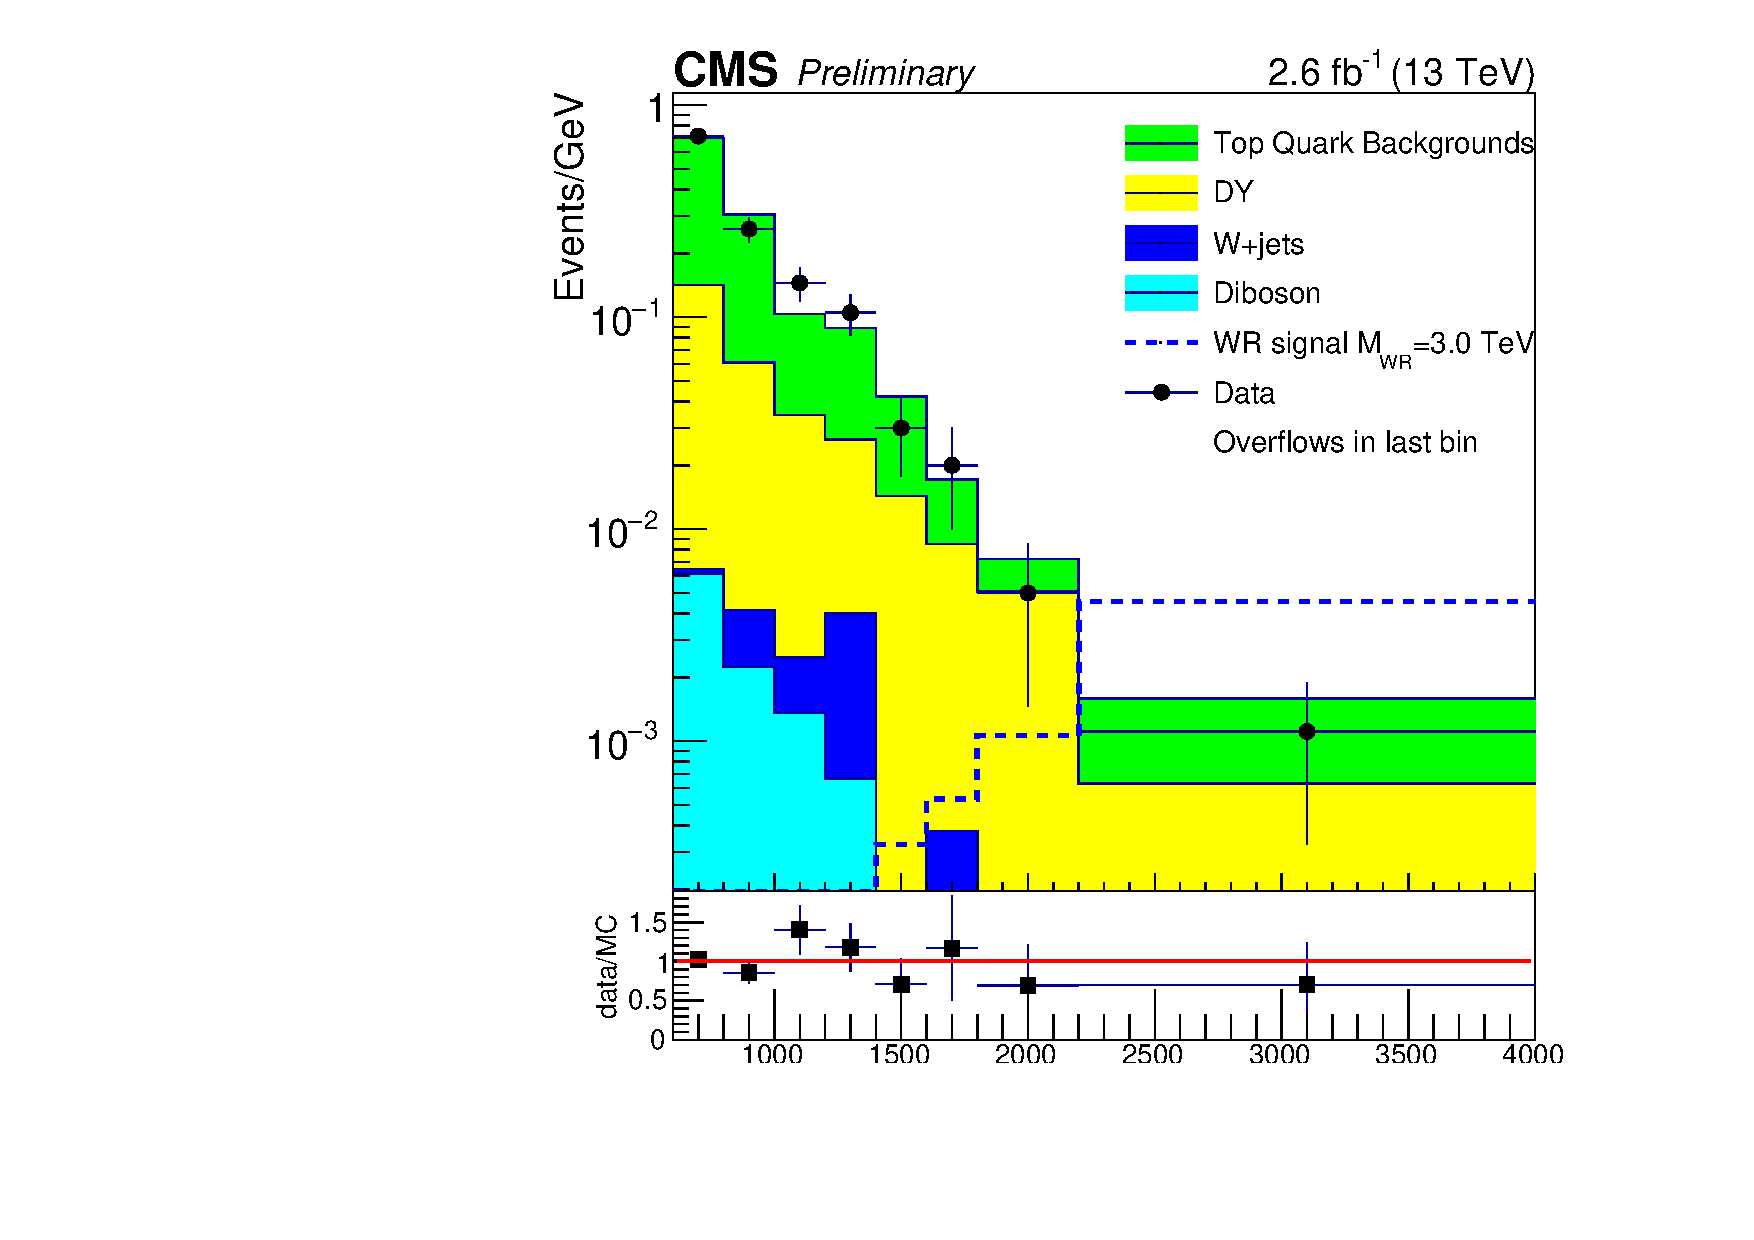
\includegraphics[width=0.65\textwidth]{figures/Mlljj_2012Bins_MWR3000Signal_SignalRegion_EEChannelBkgndMC_DYMadHTAndIncl_TTBarFromData_WithUnblindedData_withRatio_log.pdf}
	}
	\subfigure{
		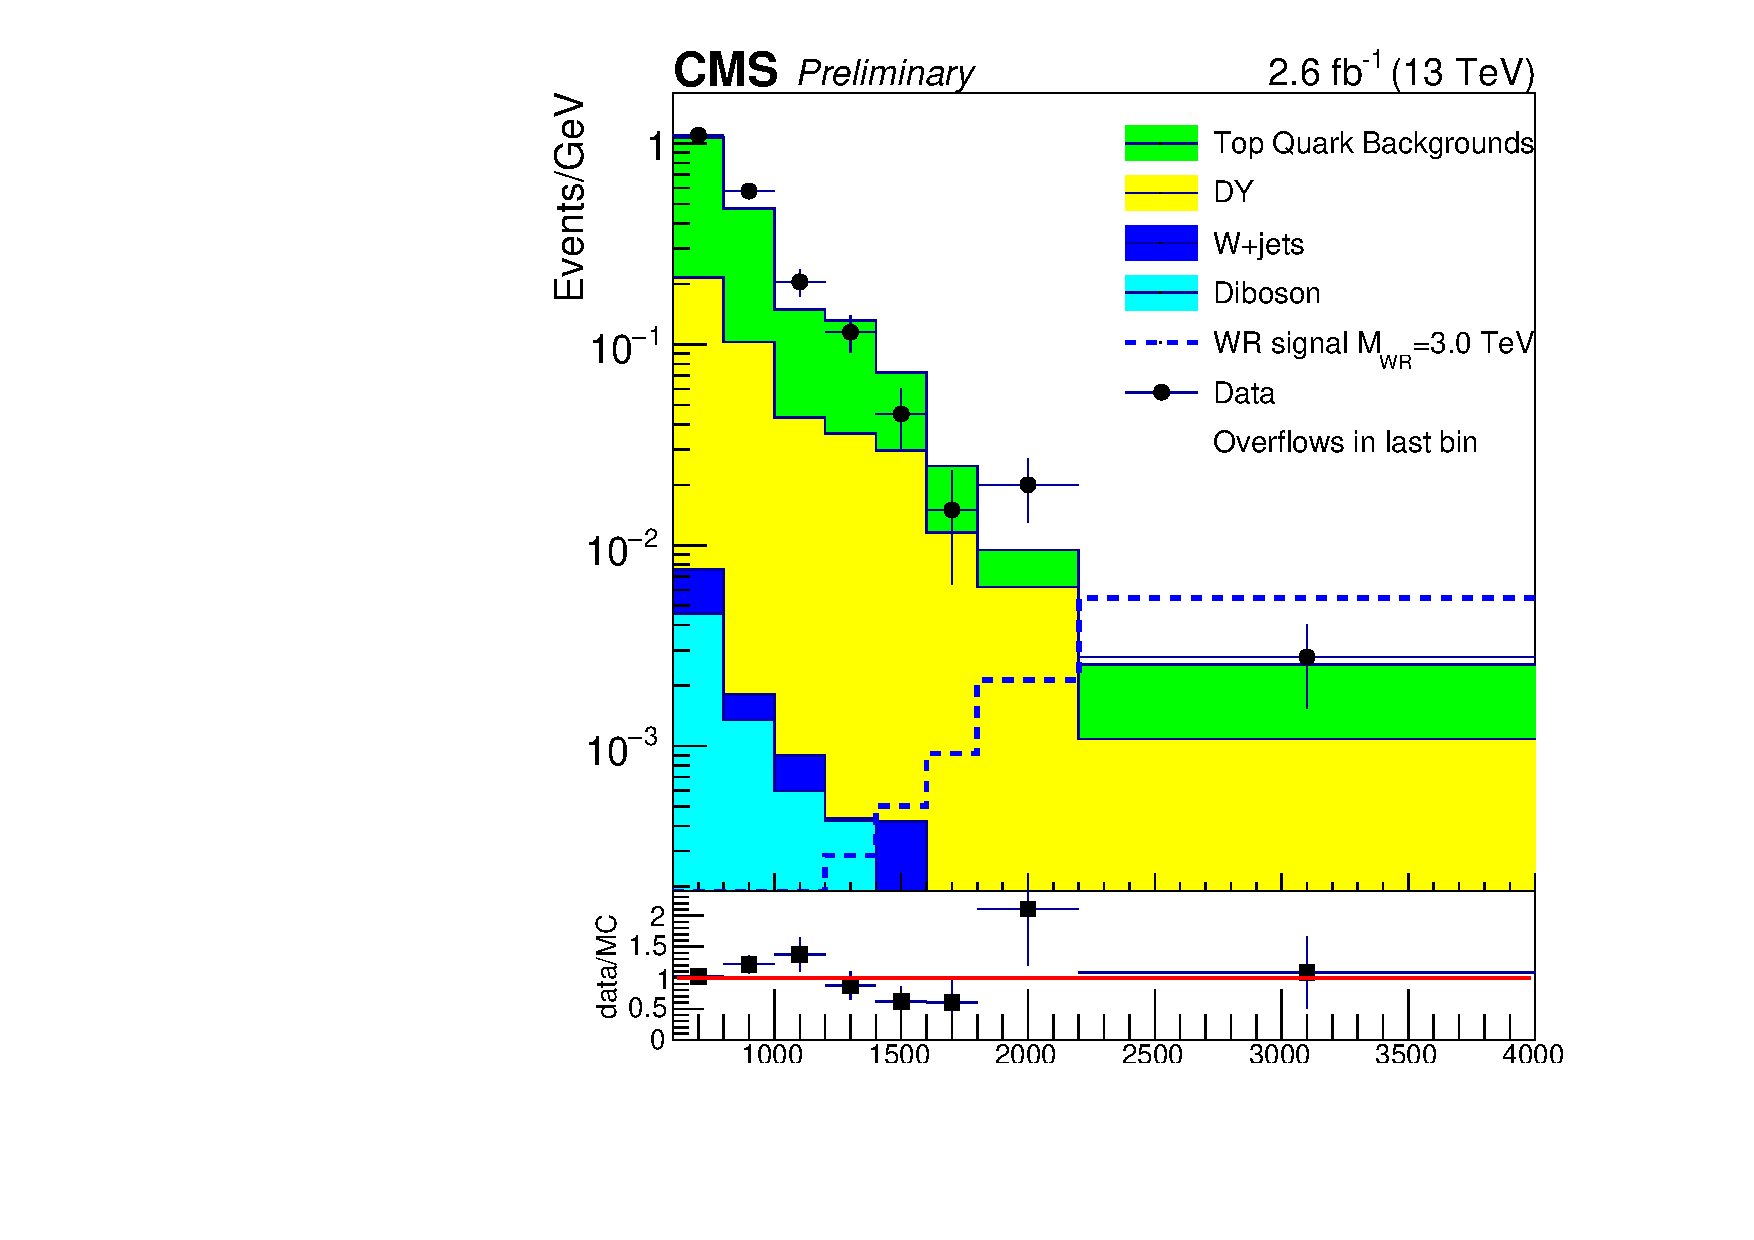
\includegraphics[width=0.65\textwidth]{figures/Mlljj_2012Bins_MWR3000Signal_SignalRegion_MuMuChannelBkgndMC_DYMadHTAndIncl_TTBarFromData_WithUnblindedData_withRatio_log.pdf}
	}
	\label{fig:obsAndExpMlljj}
	\caption{The $\Mlljj$ distributions after selections found in data, \WR simulations, and expected backgrounds.  The $ee$ ($\mu\mu$) 
		channel is shown on the left (right).}
\end{figure}

Upper limits on $\sigma(\WR) \times BR(\WR \rightarrow \ell\ell jj)$ were calculated at 95\% CL in each $\Mlljj$ window 
assuming $\mnul = \frac{1}{2}\mWR$.  Expected limits were calculated by setting the measured number of events $\Nlljj$ 
equal to the number of ST background events, and observed limits were calculated by setting $\Nlljj$ equal to the number 
of events found in data.  The expected and observed limits as functions of \mWR are shown in Figure \ref{fig:oneDimLimits}.  
Subsequently, the expected and observed cross section limits for $\mnul = \frac{1}{2}\mWR$ were extrapolated into \mnul 
and \mWR exclusion limits.

\begin{figure}[btp]
	\centering
	\subfigure{
		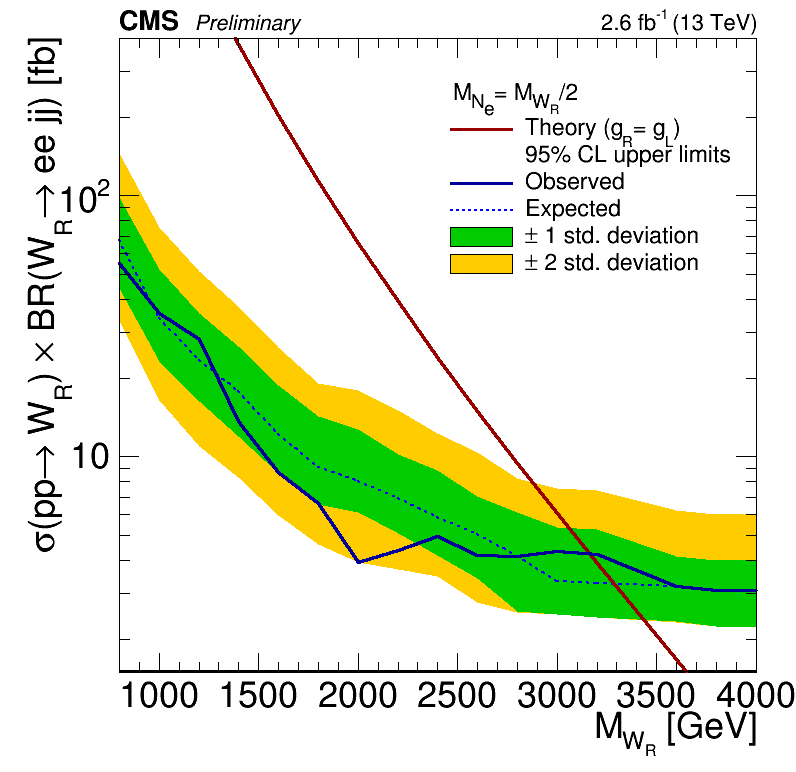
\includegraphics[width=0.65\textwidth]{figures/limWReejj_SHv19700toysAprilTwentyThree.png}
	}
	\subfigure{
		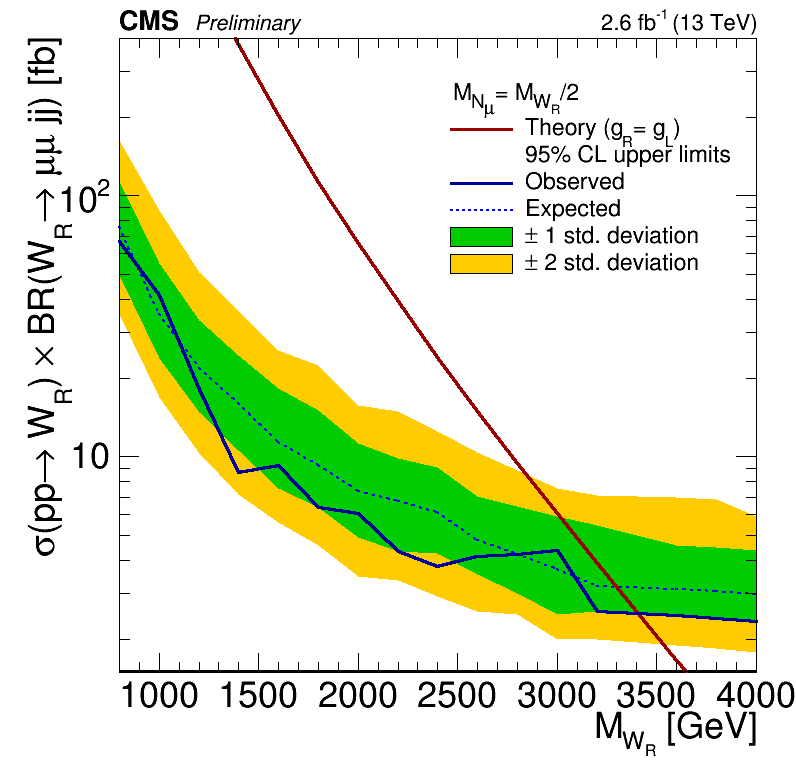
\includegraphics[width=0.65\textwidth]{figures/limWRmumujj_SHv19700toysAprilTwentyThree.png}
	}
	\label{fig:oneDimLimits}
	\caption{Limits on $\sigma(\WR) \times BR(\WR \rightarrow \ell\ell jj)$ at 95\% CL versus \mWR hypothesis.  The $ee$ ($\mu\mu$) channel 
	is shown on the left (right).}
\end{figure}

The limits on $\sigma(\WR) \times BR(\WR \rightarrow \ell\ell jj)$ for any \mnul were linearly proportional to the signal 
efficiency $\chi$ of the event selection multiplied by the \WR cross section $\sigma(\WR)$, $\chi \times \sigma(\WR)$.  
Since the estimated background was only sensitive to the \mWR hypothesis, the limits at two points with the same \mWR but 
different \mnul only differed by the ratio of $\chi \times \sigma(\WR)$ at the points.  Since the $\sigma(\WR) \times BR(\WR \rightarrow \ell\ell jj)$ 
limit was known at $(\mWR^{a}, \mnul^{a} = \frac{1}{2}\mWR^{a})$, the limit at any other point $(\mWR^{a}, \mnul^{b} \neq \frac{1}{2}\mWR^{a})$ 
could be calculated as:

\begin{equation}
	Limit[(\mWR^{a}, \mnul^{b} \neq \frac{1}{2}\mWR^{a})] = \frac{\chi[(\mWR^{a}, \mnul^{b} \neq \frac{1}{2}\mWR^{a})]}{\chi[(\mWR^{a}, \mnul^{a} = \frac{1}{2}\mWR^{a})]} \quad Limit[(\mWR^{a}, \mnul^{a} = \frac{1}{2}\mWR^{a})]
\label{eq:limitExtrapolation}
\end{equation}
The dependence of $\chi$ on \mnul and \mWR was estimated by simulating additional $\WR \rightarrow \ell\ell jj$ samples with 
\mWR increasing from 800 to 4000 $\GeV$ in 100 $\GeV$ steps.  At each \mWR value, at least 20 samples were produced with 
different \mnul values between 0 $\GeV$ and \mWR.  
%in steps of:
%\begin{itemize}
%	\item 25 $\GeV$ from 0 to 300 $\GeV$,
%	\item 100 $\GeV$ from 300 to $\mWR - 200$ $\GeV$,
%	\item 25 $\GeV$ from $\mWR - 200$ to \mWR $\GeV$
%\end{itemize}
%Smaller steps were used in regions where $\chi$ had a strong dependence on \mnul.
The standard full simulation and reconstruction used to produce \WR samples with $\mnul = \frac{1}{2}\mWR$ required enormous 
computational resources that were not available for the limit extrapolation procedure described here.  Instead, additional \WR 
simulations were produced using only the first simulation step.  \PYTHIA simulated the \WR production and decay into leptons 
and quarks, and the hadronization of quarks into jets.  Similar to reconstructed jets, jets from \PYTHIA were clustered from 
individual hadrons, leptons and photons in a cone of radius $\Delta R =$ 0.4.  After jet clustering, the offline selection was 
applied, excluding lepton and jet ID selections.  The efficiency of this selection $\chi^'$ was measured as a function of 
$(\mWR, \mnul)$, and used in place of $\chi$.  Then, $\chi^'$ and Equation \ref{eq:limitExtrapolation} were used to extrapolate 
the $\sigma(\WR) \times BR(\WR \rightarrow \ell\ell jj)$ limits calculated for $\mnul = \frac{1}{2}\mWR$ to new limits $L'$ for 
$\mnul \neq \frac{1}{2}\mWR$.  The resulting $\sigma(\WR) \times BR(\WR \rightarrow \ell\ell jj)$ limits were rescaled by $\sigma(\WR)$ 
for $\mnul \neq \frac{1}{2}\mWR$ to obtain the \mnul and \mWR exclusion limits at 95\% CL shown in Figure \ref{fig:twoDimLimits}.

\begin{figure}[tp]
  \centering
  
  \subfigure{
    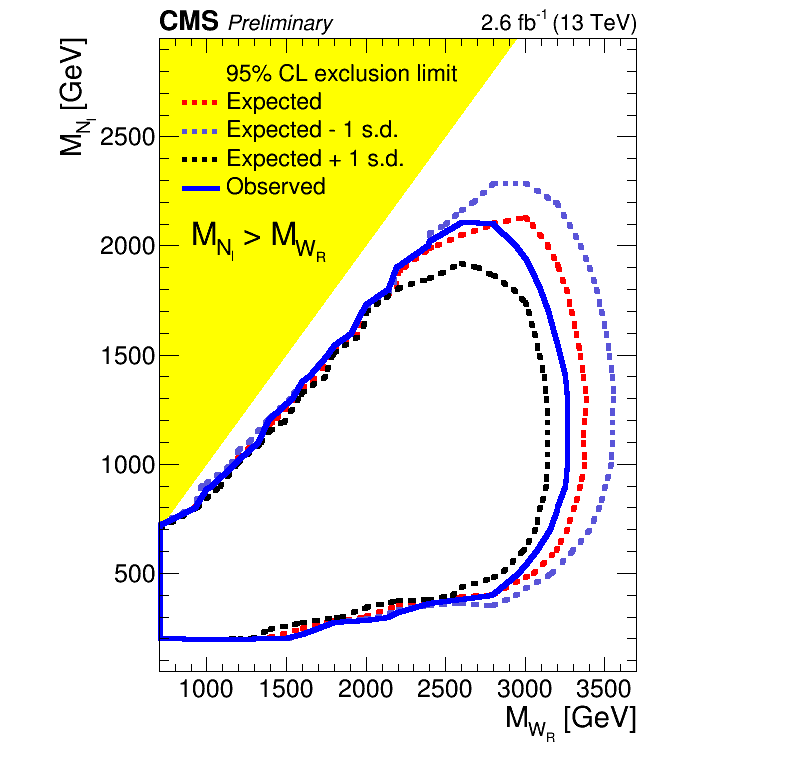
\includegraphics[width=0.65\textwidth]{figures/lim2dWReejj_SHv19700toysAprilTwentyThree_exclusionOverlayWithExpPlusMinusOneSigma.png}
  }
  \subfigure{
    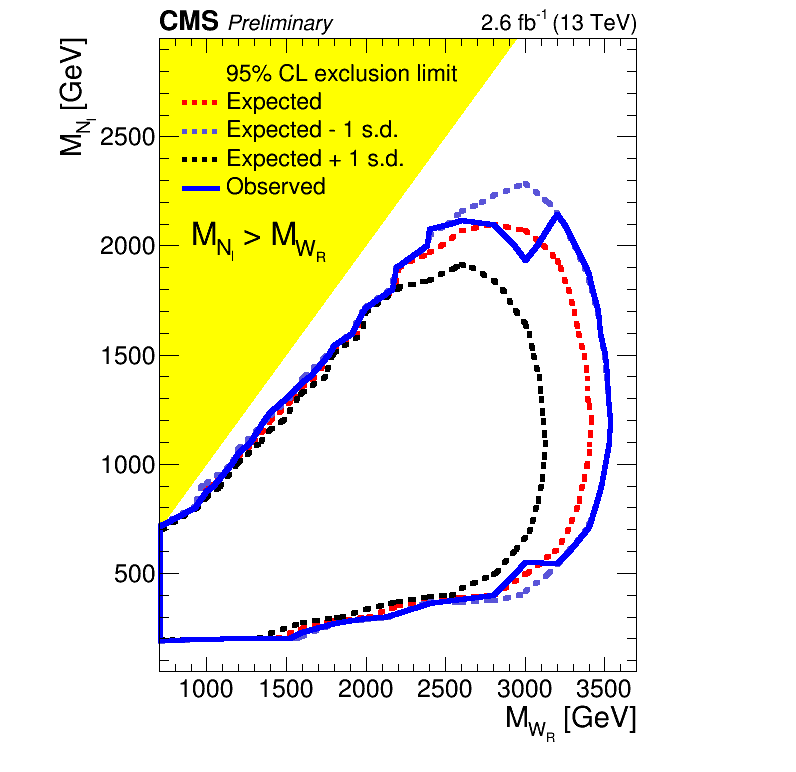
\includegraphics[width=0.65\textwidth]{figures/lim2dWRmumujj_SHv19700toysAprilTwentyThree_exclusionOverlayWithExpPlusMinusOneSigma.png}
  }
  \caption{The exclusion limits on \mWR and \mnul at 95\% CL for $\WR \rightarrow eejj$ (left) and $\WR \rightarrow \mu\mu jj$ (right).}
  \label{fig:twoDimLimits}
 
\end{figure}

The difference between the selection efficiencies $\chi^'$, without reconstruction, and $\chi$ was estimated by simulating 
$\WR \rightarrow \ell\ell jj$ at $\mWR =$ 2400 and 4000 $\GeV$ and several $\mnul \neq \frac{1}{2}\mWR$ with detector 
response simulations and particle reconstruction, and calculating limits with these events.  Simulated events were selected with the online and offline selection 
requirements, and the limits $L_{true}$ on $\sigma(\WR) \times BR(\WR \rightarrow \ell\ell jj)$ were calculated at each 
$(\mWR, \mnul \neq \frac{1}{2}\mWR)$ point.  For $\mnul \gtrsim \frac{1}{8}\mWR$, $L_{true}$ and $L'$ were consistent 
within their uncertainties.  For $\mnul \lesssim \frac{1}{8}\mWR$, the limit $L_{true}$ was stronger than $L'$ because of 
pileup jets.  $L_{true}$ was calculated using simulated events that included pileup interactions, on average 10 per event, that 
produced pileup jets, which enabled more \WR events to pass the full selection.  The resulting increase in signal selection 
efficiency $\chi$ extended the excluded \WR production region to lower \mnul values.  Although $\chi > \chi^'$ in this region, 
both signal selection efficiencies were below 10\%, and at every \mWR value the difference in the lowest excluded \mnul between 
$L_{true}$ and $L'$ was less than 100 $\GeV$.  The extrapolated limit $L'$ represented the result, and no correction was applied 
to it because $L'$ was weaker than $L_{true}$.


%%%%%%%%%%%%%%%%%%%%%%%%%%%%%%%%%%%%%%%%%%%%%%%%%%%%%%%%%%%%%%%%%%%%%%%%%%%%%
